%% LaTeX Beamer presentation template (requires beamer package)
%% see http://latex-beamer.sourceforge.net/
%% idea contributed by H. Turgut Uyar
%% template based on a template by Till Tantau
%% this template is still evolving - it might differ in future releases!

\documentclass{beamer}
\usepackage[brazil]{babel}
\usepackage[utf8]{inputenc}
\usepackage{amsfonts}
\usepackage{amsmath}

\mode<presentation>
{
    \usetheme{PaloAlto}
    
    \setbeamercovered{transparent}
}


\title{Reconhecimento e localização de pessoas em um SmartSpace}
%\subtitle{}

% - Use the \inst{?} command only if the authors have different
%   affiliation.
\author{Tales Porto e Danilo Ávila}
%\author{\inst{1}}

% - Use the \inst command only if there are several affiliations.
% - Keep it simple, no one is interested in your street address.
\institute[UnB]
{
    %\inst{1}%
    Instituto de Ciências Exatas\\
    Departamento de Ciência da Computação\\
    Universidade de Brasília
}

\date{20 de junho de 2011}


% This is only inserted into the PDF information catalog. Can be left
% out.
%\subject{Talks}



% If you have a file called "university-logo-filename.xxx", where xxx
% is a graphic format that can be processed by latex or pdflatex,
% resp., then you can add a logo as follows:

% \pgfdeclareimage[height=0.5cm]{university-logo}{university-logo-filename}
% \logo{\pgfuseimage{university-logo}}



% Delete this, if you do not want the table of contents to pop up at
% the beginning of each subsection:
%\AtBeginSubsection[]
%{
%\begin{frame}<beamer>
%    \frametitle{Sumário}
%    \tableofcontents[currentsection,currentsubsection]
%    \end{frame}
%}

% If you wish to uncover everything in a step-wise fashion, uncomment
% the following command:

%\beamerdefaultoverlayspecification{<+->}

\begin{document}

% ------------- TITLE PAGE -------------
\begin{frame}
\titlepage
\end{frame}
% ------------- TITLE PAGE -------------


% ------------- SUMARIO -------------
\begin{frame}
	\frametitle{Sumário}
	\tableofcontents
\end{frame}


% ------------- Introdução -------------
\section{Introdução}

% ------------- Contexto -------------
\subsection{Contexto}

\begin{frame}
    \frametitle{Computação Ubíqua}

	\begin{itemize}
  		\item Tem como objetivo tornar a interação pessoa-máquina invisível, ou seja, integrar a informática com as ações e comportamentos naturais das pessoas.
	\end{itemize}

    \begin{figure}[h]
    	\centering 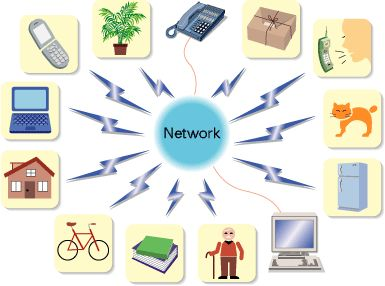
\includegraphics[scale=0.9]{figuras/ubiquitous.gif}
    	\caption{Esquema de computação ubíqua}
	\label{esquema_computacao_ubiqua} 
    \end{figure}
\end{frame}

\begin{frame}
    \frametitle{SmartSpace}

    SmartSpaces são espaços onde a computação ubíqua acontece em sua quase totalidade.
    
    \begin{figure}[h]
    	\centering 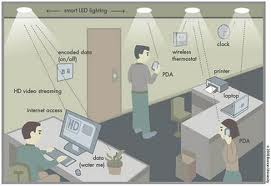
\includegraphics[scale=0.35]{figuras/smartSpace.jpg}
    	\caption{Smart Space}
    	\label{smart_space} 
    \end{figure}
\end{frame}

\begin{frame}
    \frametitle{Reconhecimento Facial}
    
    \begin{figure}[h]
	\centering 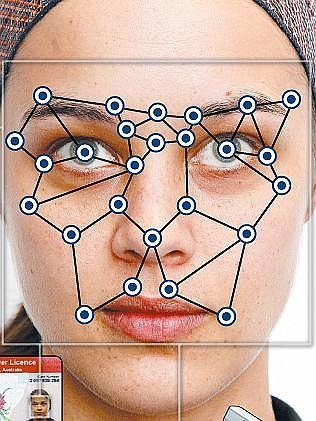
\includegraphics[scale=0.4]{figuras/face-recognition.jpg}
    	\caption{Exemplo de reconhecimento facial}
    	\label{reconhecimento_facial}
    \end{figure}
\end{frame}

% ------------- Problema -------------
\section{Problema}
\begin{frame}
    \frametitle{Problema}
    Reconhecer em tempo real os usuários presentes no SmartSpace e rastrear-los durante a sua permanência. \\
	\begin{itemize}
      		\pause \item Deve ser ter um índice de confiança mínimo de --095\% no reconhecimento. \\
		\pause \item Os usuários iram se identificar(cadastrar) somente na primeira vez que entrar no SmarSpace. \\
    		\pause \item O processo recolherá informações de contexto do usuário e disponibilizará para o middleware chamado \it{UnBiquitous}.
	\end{itemize}
\end{frame}

\section{Justificativa} 
\begin{frame}
    \frametitle{Justificativa}
    \begin{itemize}
      \item Aumento no rendimento dos dipositivos, já que haverá economia de
      energia
      \item Diminui-se os custos, já que pode-se tirar o elemento centralizador
      da infraestrutura.
    \end{itemize}
\end{frame}


% ------------- SOBRE O TRABALHO -------------
\section{Sobre o Trabalho}
\begin{frame}
    \frametitle{Sobre o Trabalho}
    \begin{itemize}
        \item Como será executado?
        \item Qual a metodologia?
    \end{itemize}
\end{frame}
% ------------- SOBRE O TRABALHO -------------


\subsection{Problema}
\begin{frame}
    \frametitle{Problema}
    Escolher um grupo $n$ dado um conjunto $N$ de nós, em que ($n$ $\leqslant$
    $N$), de modo que este subgrupo possa executar uma determinada ação num determinado momento.
\end{frame}


\subsection{Hipótese}
\begin{frame}
    \frametitle{Hipóteses}
    \begin{itemize}
      \item É possível encontrar uma política de seleção que seja rápida e
      maximize a economia de energia, sem prejudicar a justiça e a execução da
      ação(por exemplo, transmissão de dados).
      \item Cenário:
        \begin{itemize}
            \item Tem-se $N$ nós
            \item Temos um subgrupo de $n$ nós que podem executar determinada
            ação num determinado tempo
            \item Este grupo não é necessariamente único
            \item Sujeito a problemas de identificação dos nós
        \end{itemize} 
    \end{itemize}
\end{frame}


\subsection{Objetivos e Resultados Esperados}
\begin{frame}
    \frametitle{Objetivos e Resultados Esperados}
    \begin{itemize}
      \item \textbf{Objetivo Geral}
        \begin{itemize}
          \item Analisar os métodos existente e propor uma solução de política
          eficiente
        \end{itemize}
      \item \textbf{Objetivo Específico}
        \begin{itemize}
          \item Propor uma solução eficiente e validá-la através de um simulador
          que será desenvolvido.
        \end{itemize}
      \item \textbf{Resultados Esperados}
        \begin{itemize}
          \item Proposta de política que:
            \begin{itemize}
              \item seja maximizado a economia de energia
              \item seja rápida
              \item seja justa
              \item seja maximizado a vazão de dados
            \end{itemize}
        \end{itemize}
    \end{itemize}
\end{frame}


\subsection{Metodologia}
\begin{frame}
    \frametitle{Metodologia}
    \begin{itemize}
    \pause \item Levantamento do estado da arte
        \begin{itemize}
            \item Identificação de problemas e pontos em aberto
        \end{itemize}
    \pause \item Proposta de solução
    \pause \item Desenvolvimento de um simulador
    \pause \item Validar solução
        \begin{itemize}
            \item Utilizando o simulador, executar coleta de dados para análise
                e validação da proposta de solução para uma política de seleção
        eficiente
        \end{itemize}
    \end{itemize}
\end{frame}


\subsection{Cronograma}
\begin{frame}
    \frametitle{Cronograma}
    \begin{itemize}
        \item Julho: Levantamento do estado da arte
        \item Agosto: Levantamento do estado da arte
        \item Setembro: Desenvolvimento do simulador
        \item Outubro: Término do desenvolvimento e coleta de dados
        \item Novembro: Análise de resultados e aspectos finais
        \item Dezembro: Apresentação
    \end{itemize}
\end{frame}


% ------------- REFERENCIAS -------------

\nocite{Stevenson09,Cordeiro04,Cormen94,Kurose2005,Stevens94,Tanenbaum03,Zimmermann80,Bae09,Jung08,Park97}

\section{Referências}

\frame[allowframebreaks]{
  \frametitle{Referências}
  \bibliographystyle{plain}
  \bibliography{bibliografia}
}

\begin{frame}
    \frametitle{ }
    \centerline{Obrigado!}
\end{frame}

\end{document}
